








  In the following diagram, what is $\sin(x)\cos(x)$?
\begin{center}
 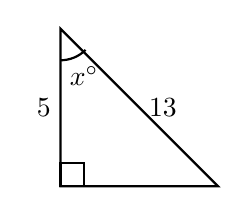
\begin{tikzpicture}
 
 \draw (0,0) --(2,0)--(0,2)--cycle  [thick,-,>=latex];
 \draw (0,0) --(0,.3)--(.3,.3)--(.3,0)--cycle  [thick,-,>=latex];
\draw[thick] (0,1.60) arc (270:315:.45);

  \draw node[below] at (.3,1.65) {$x^\circ$};
  \draw node[left] at (0,1) {$5$};
   \draw node[right] at (1,1) {$13$};
\end{tikzpicture}
\end{center}




\ifsat
	\begin{enumerate}[label=\Alph*)]
		\item  $\frac{12}{13}$ 
		\item $\frac{60}{13}$ 
		\item  $\frac{60}{169}$ %
		\item Cannot be determined
	\end{enumerate}
\else
\fi

\ifacteven
	\begin{enumerate}[label=\textbf{\Alph*.},itemsep=\fill,align=left]
		\setcounter{enumii}{5}
		\item    $\frac{5}{13}$
		\item  $\frac{12}{13}$ 
		\item $\frac{60}{13}$ 
		\addtocounter{enumii}{1}
		\item  $\frac{60}{169}$ %
		\item Cannot be determined
	\end{enumerate}
\else
\fi

\ifactodd
	\begin{enumerate}[label=\textbf{\Alph*.},itemsep=\fill,align=left]
		\item    $\frac{5}{13}$
		\item  $\frac{12}{13}$ 
		\item $\frac{60}{13}$ 
		\item  $\frac{60}{169}$ %
		\item Cannot be determined
	\end{enumerate}
\else
\fi

\ifgridin
  $\frac{60}{169}$ %
		
\else
\fi

